\documentclass[14pt,xcolor=dvipsnames,table,dvipdfmx]{beamer}

\setbeamertemplate{bibliography item}[text]
\usepackage[absolute,overlay]{textpos}
\usepackage{apalike}
\usetheme{Boadilla}

\usepackage{txfonts} % TXフォント
\renewcommand{\kanjifamilydefault}{\gtdefault}  % 日本語をゴシック体に
\usefonttheme{structurebold} % タイトル部を太字
\setbeamerfont{alerted text}{series=\bfseries} % Alertを太字
\setbeamerfont{section in toc}{series=\mdseries} % 目次は太字にしない
\setbeamerfont{frametitle}{size=\Large} % フレームタイトル文字サイズ
\setbeamerfont{title}{size=\LARGE} % タイトル文字サイズ
\setbeamerfont{date}{size=\small}  % 日付文字サイズ
\usepackage{pxjahyper}

\uselanguage{japanese}
\languagepath{japanese}
\deftranslation[to=japanese]{Theorem}{定理}
\deftranslation[to=japanese]{Lemma}{補題}
\deftranslation[to=japanese]{Example}{例}
\deftranslation[to=japanese]{Examples}{例}
\deftranslation[to=japanese]{Definition}{定義}
\deftranslation[to=japanese]{Definitions}{定義}
\deftranslation[to=japanese]{Problem}{問題}
\deftranslation[to=japanese]{Solution}{解}
\deftranslation[to=japanese]{Fact}{事実}
\deftranslation[to=japanese]{Proof}{証明}
\def\proofname{証明}

\definecolor{UniBlue}{RGB}{0,150,200} 
\definecolor{AlertOrange}{RGB}{255,76,0}
\definecolor{AlmostBlack}{RGB}{38,38,38}
\setbeamercolor{normal text}{fg=AlmostBlack}  % 本文カラー
\setbeamercolor{structure}{fg=UniBlue} % 見出しカラー
\setbeamercolor{block title}{fg=UniBlue!50!black} % ブロック部分タイトルカラー
\setbeamercolor{alerted text}{fg=AlertOrange} % \alert 文字カラー
\mode<beamer>{
    \definecolor{BackGroundGray}{RGB}{254,254,254}
    \setbeamercolor{background canvas}{bg=BackGroundGray} % スライドモードのみ背景をわずかにグレーにする
}

% Algorithm系
\usepackage{algorithm}
\usepackage[noend]{algorithmic}
\algsetup{linenosize=\color{fg!50}\footnotesize}
\renewcommand\algorithmicdo{:}
\renewcommand\algorithmicthen{:}
\renewcommand\algorithmicrequire{\textbf{Input:}}
\renewcommand\algorithmicensure{\textbf{Output:}}

%フラットデザイン化
\setbeamertemplate{blocks}[rounded] % Blockの影を消す
\useinnertheme{circles} % 箇条書きをシンプルに
\setbeamertemplate{navigation symbols}{} % ナビゲーションシンボルを消す
\setbeamertemplate{footline}[frame number] % フッターはスライド番号のみ

\AtBeginSection[]{
    \frame{\tableofcontents[currentsection, hideallsubsections]} %目次スライド
}

\title{\bfseries 質問者のプライバシーを保護する特許デーだベース検索(研究紹介)}
%\subtitle{\bfseries ─ 講演用スライド作成のために ─}
\date{2016年7月1日}
\author{中川研M2 胡 瀚林 \\ 指導教員:中川 裕志 教授}
%\subject{PIR}
%\keywords{PIR,Obfuscation,query}

\begin{document}

\maketitle
\frame{\tableofcontents[hideallsubsections]}

\section{背景紹介}
\begin{frame}{特許検索}
\begin{columns}[t]
    \begin{column}{0.8\textwidth} % 横幅の30%
      	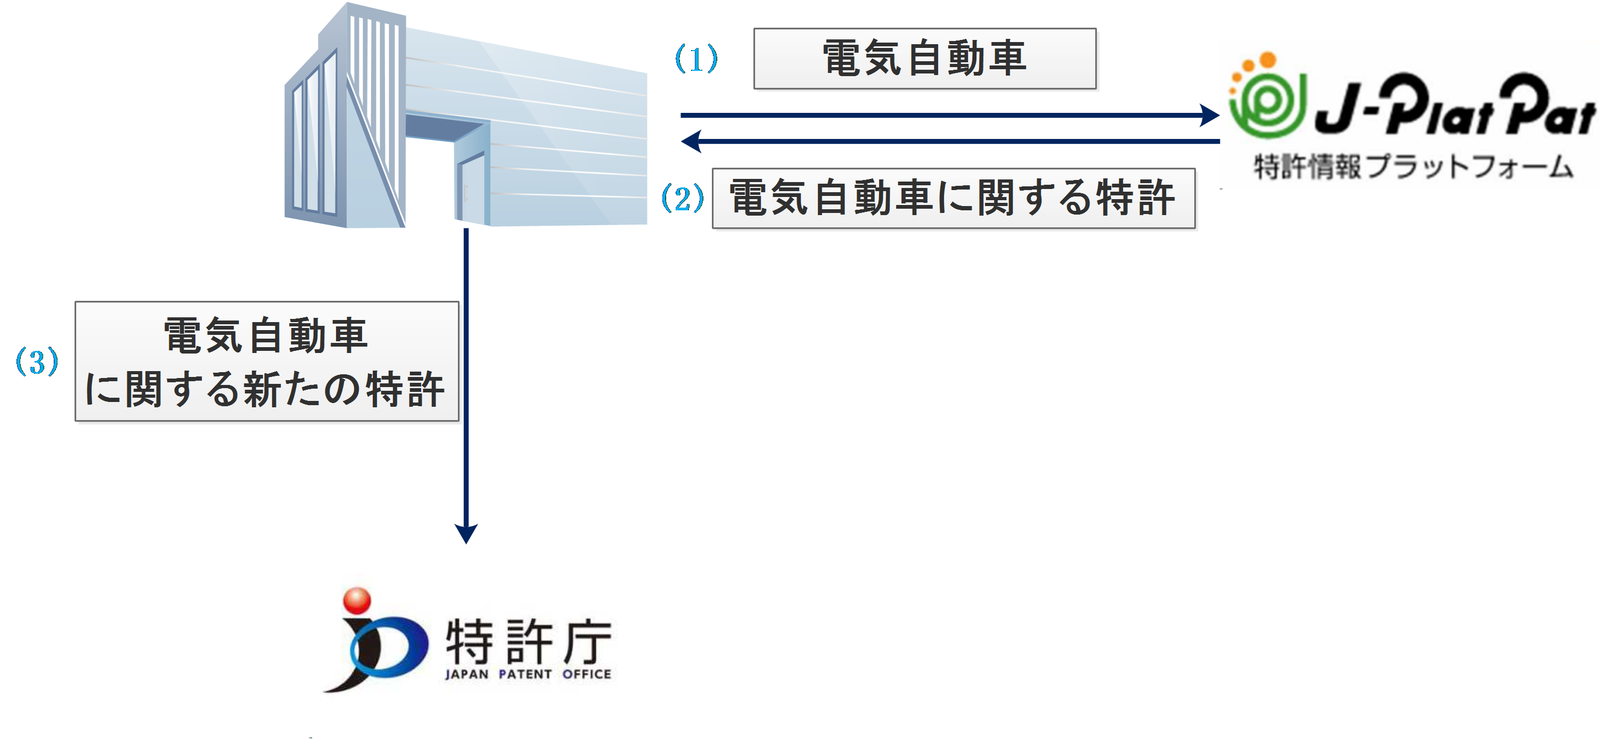
\includegraphics[width=\columnwidth]{rk1.png}
    \end{column}
\end{columns}
\end{frame}

\begin{frame}{特許検索}
\begin{columns}[t]
    \begin{column}{0.8\textwidth} % 横幅の30%
      	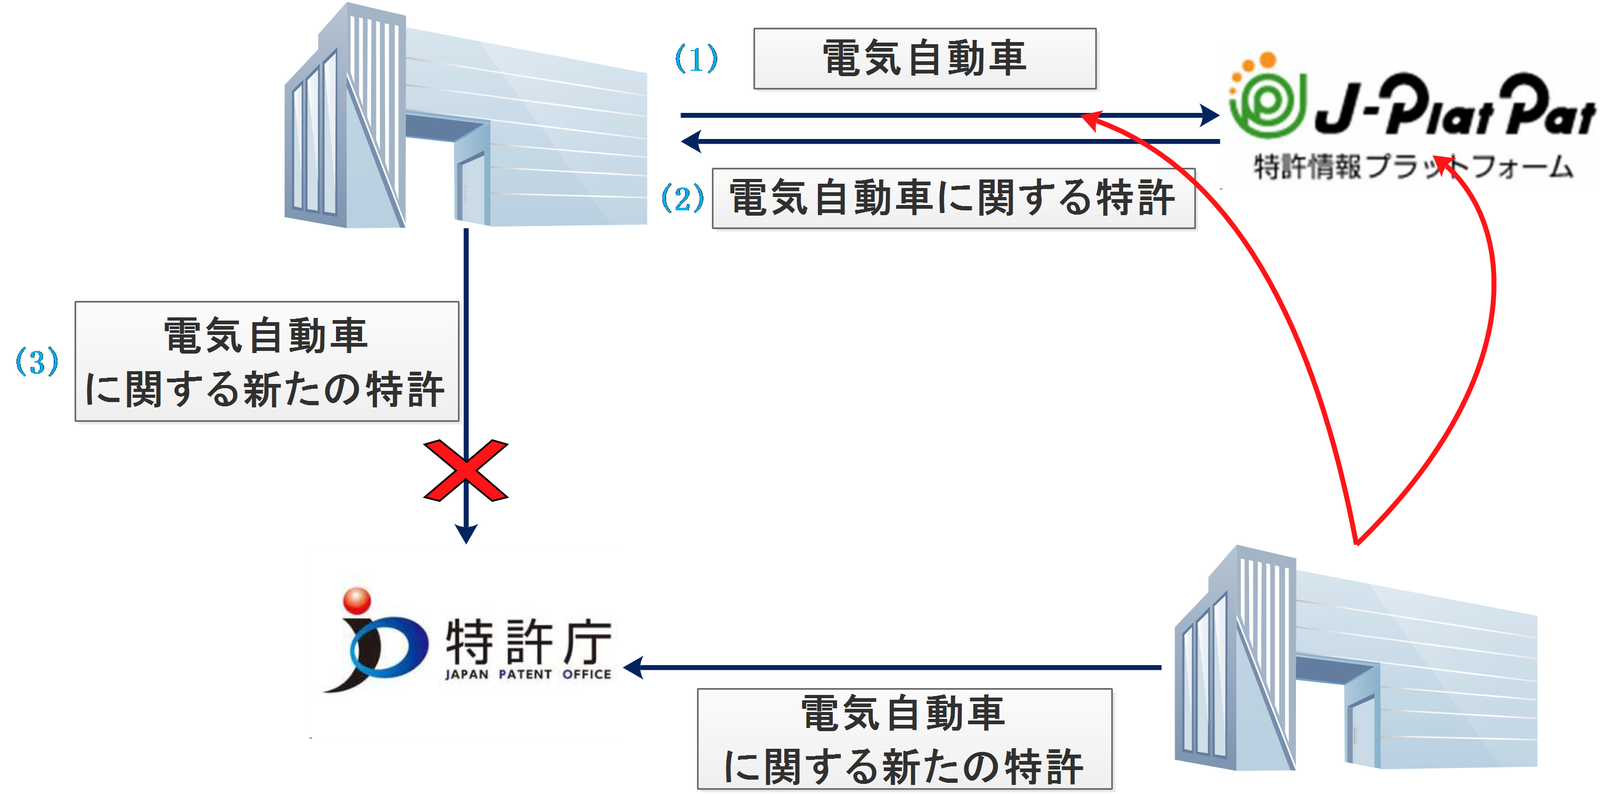
\includegraphics[width=\columnwidth]{rk2.png}
    \end{column}
\end{columns}
\end{frame}

\begin{frame}{質問ベース検索}
\begin{columns}[t]
    \begin{column}{0.8\textwidth} % 横幅の30%
        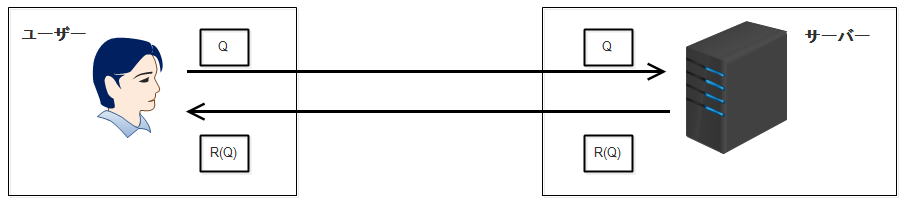
\includegraphics[width=\columnwidth]{photo1.png}
    \end{column}
\end{columns}
    \begin{block}{}
    \begin{itemize}
        \item Q:検索質問
        \item R(Q):質問Qの検索結果
    \end{itemize}
    \end{block}
\end{frame}

\begin{frame}{Obfuscation Search}
    \begin{columns}[t]
        \begin{column}{1\textwidth} % 横幅の30%
            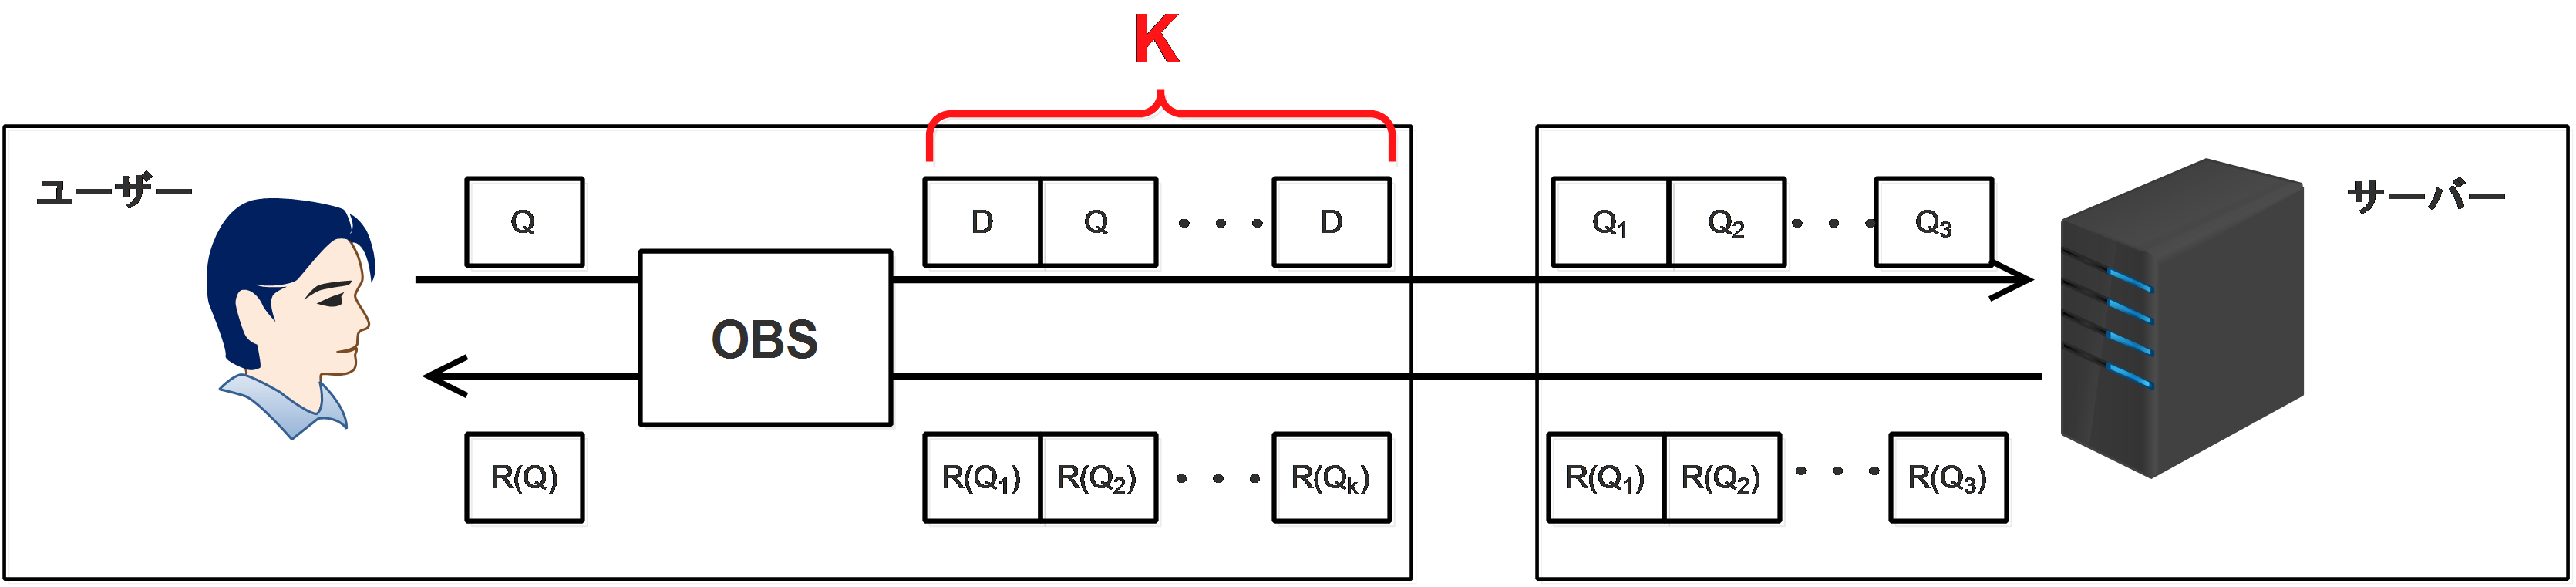
\includegraphics[width=\columnwidth]{rk4.png}
		\end{column}
    \end{columns}
	\begin{block}{} 
		\begin{itemize}
			\item 複数の質問を混ぜて検索する
		\end{itemize}
	\end{block}
\end{frame}

\begin{frame}{Prive Information Retrieval\cite{ostrovsky_survey_2007}}
	\begin{columns}[t]
		\begin{column}{0.8\textwidth} % 横幅の30%
			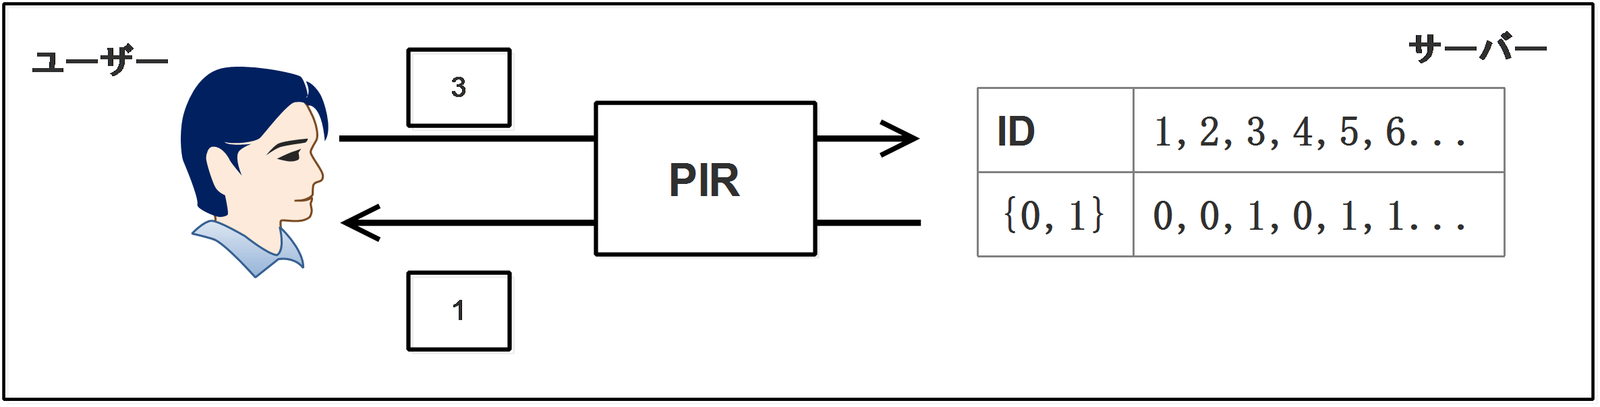
\includegraphics[width=\columnwidth]{rk5.png}
		\end{column}
	\end{columns}
	\begin{block}{} 
		\begin{itemize}
			\item 暗号などの手法を用いて質問の内容を完全に隠す
		\end{itemize}
	\end{block}
\end{frame}

\begin{frame}{凖同型暗号}
	\begin{Definition}[凖同型暗号]
		二つの暗号文 $Enc(m_1), Enc (m_2)$ が与えられた時に、平文や秘密鍵なしで $Enc( m_1 \circ m_2 )$ を計算できる暗号
	\end{Definition}
	\begin{Example}[加算ができる凖同型暗号]
		$Enc(\cdot):$ 暗号化 \, $Dec(\cdot):$復号 \\
		$ Dec(Enc(m_1) \cdot Enc (m_2)) = m_1 + m_2$
	\end{Example}
\end{frame}
\begin{frame}{凖同型暗号}
\fontsize{12pt}{7.2}\selectfont
    \begin{columns}[t]
        \begin{column}{0.5\textwidth}
			\begin{block}{ユーザー} 
			\begin{columns}[t]
				\begin{column}{0.8\textwidth}
				\begin{block}{質問生成}
				\begin{algorithmic}[1]
					\STATE Input:$i^*,n$
					\FOR{$i = 1, \dots, n$}
					\IF{$i == i^*$}
					\STATE {$ q_i = Enc(1)$}
					\ELSE
					\STATE{$ q_i =Enc(0)$}
					\ENDIF
					\ENDFOR
					\RETURN $Q = \{q_1, \dots, q_n\}$
				\end{algorithmic}
				\end{block}
				\begin{block}{復号}
				\begin{algorithmic}[1]
					\STATE input:$R$
					\RETURN $Dec(R)$
				\end{algorithmic}
				\end{block}
				\end{column}
			\end{columns}
			\end{block}
        \end{column}
        \begin{column}{0.5\textwidth}
			\begin{block}{サーバー} 
			\begin{columns}[t]
				\begin{column}{0.8\textwidth}
				\begin{block}{結果計算}
				\begin{algorithmic}[1]
					\STATE Input:$Q,\{x_1, \dots, x_n \}$
					\STATE $R = 0$
					\FOR{$i = 1, \dots, n$}
					\STATE $R = R \cdot q_i^{x_i}$
					\ENDFOR
					\RETURN $R$
				\end{algorithmic}
				\end{block}
				\end{column}
			\end{columns}
			\end{block}
			\begin{block}{Note}
				$m_1 = m_2 \nRightarrow Enc(m_1) = Enc(m_2)$ \\
				$Dec(R) = \sum_{x_i = 1}Dec(q_i) = x_{i^*}$
			\end{block}
        \end{column}
    \end{columns}
\end{frame}

\begin{frame}{性能}
	\begin{columns}[t]
	\begin{column}{0.8\textwidth}
	\begin{exampleblock}{}
    \begin{tabular}{cccc}
    \noalign{\hrule height 1pt}
     & OBS & OBS+PIR & PIR  \\
    \hline
    サーバーの協力 & 不要 & ? & 必要 \\
    安全性 & 弱い & ? & 強い \\
    スピード & 速い & ? & 遅い \\
    \noalign{\hrule height 1pt}
    \end{tabular}
	\end{exampleblock}
	\end{column}
	\end{columns}
	\begin{block}{}
		安全性はOBSより強い、スピードはPIRより速い中間手法がほしい
	\end{block}
\end{frame}

\begin{frame}{特許検索クエリ}
	\fontsize{10pt}{7.2}\selectfont
	\begin{exampleblock}{メタノールを燃料とする車載用燃料電池システムおよび車}
	メタノール 水蒸気 反応 水素 透過 膜 自立 燃料 電池 システム 供給 ガス \\ アノード カソード 空気 排出
	\end{exampleblock}
	\fontsize{14pt}{7.2}\selectfont
	\begin{block}{}
    \begin{itemize}
        \item 単語数が多い
        \item 専門用語が多い
    \end{itemize}
	\end{block}
\end{frame}

\begin{frame}{国際特許分類}
	\begin{exampleblock}{\center A61C 5/08A}
	\begin{tabular}{cc}
	セクション:A & 健康および娯楽 \\
 	サブセクション : 61 & 医学または獣医学:衛生学 \\
 	クラス: C & 歯科:口腔または歯科衛生 \\
 	メイングループ:5 & 歯の充填または被覆 \\
 	サブグループ:08 & 歯冠:その製造;口中での歯冠固定 \\
	\end{tabular}
	\end{exampleblock}
\end{frame}

\section{既存研究}
\begin{frame}{Embellishing Text Search Queries to Protect User Privacy \cite{pang_embellishing_2010}}
	\begin{columns}[t]
		\begin{column}{0.8\textwidth} % 横幅の30%
			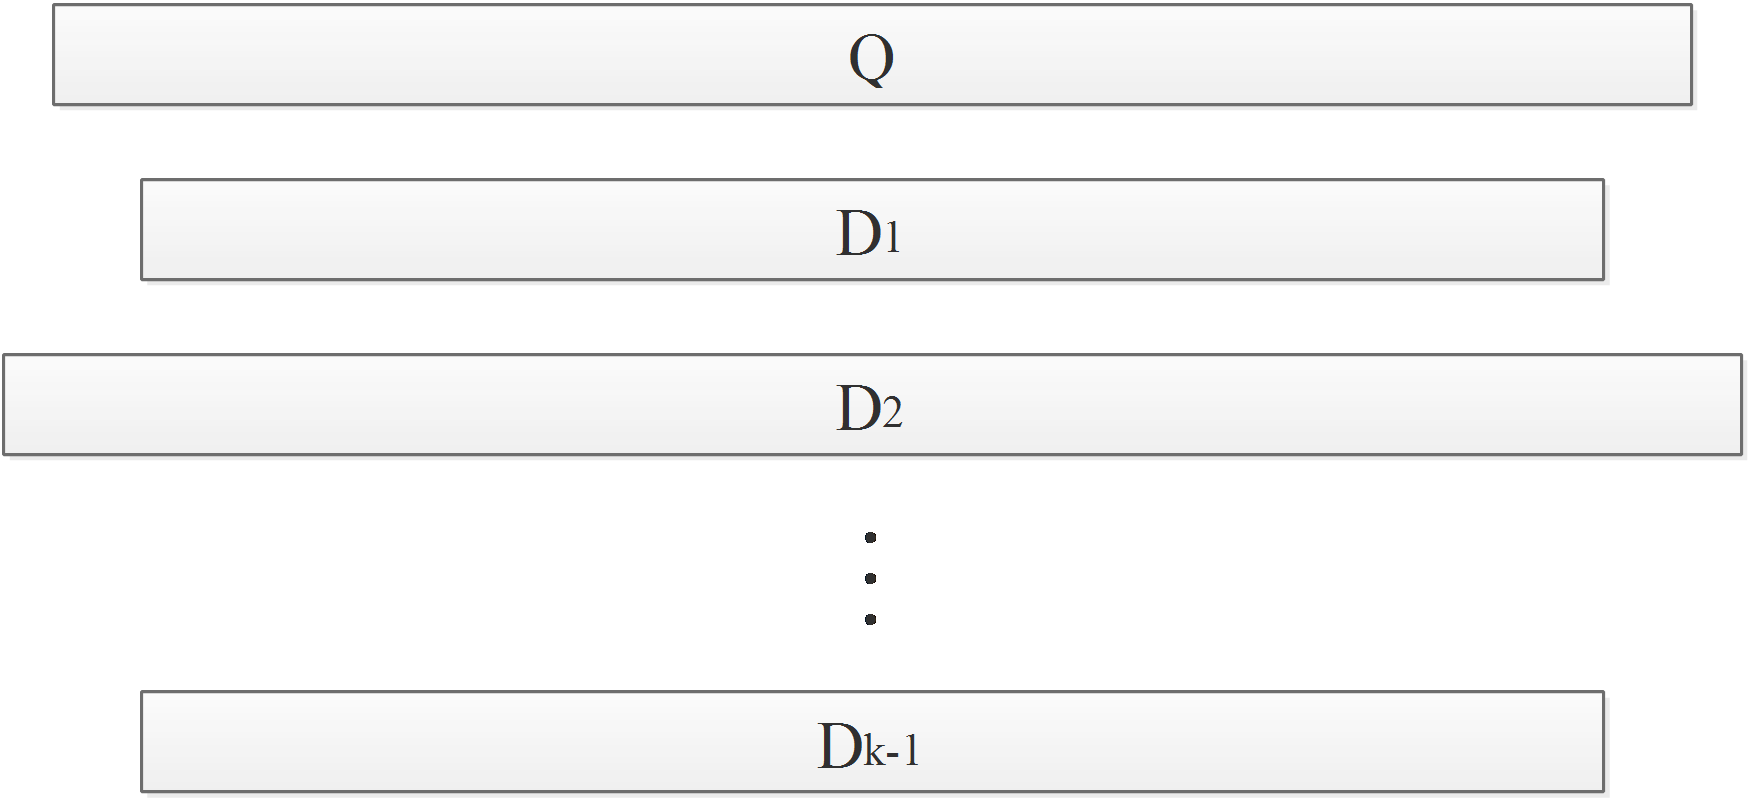
\includegraphics[width=\columnwidth]{rk6.png}
		\end{column}
	\end{columns}
	\begin{block}{}
		真の質問である可能性がある質問数:$K$	
	\end{block}
\end{frame}

\begin{frame}{ETS}
	\begin{columns}[t]
		\begin{column}{0.8\textwidth} % 横幅の30%
			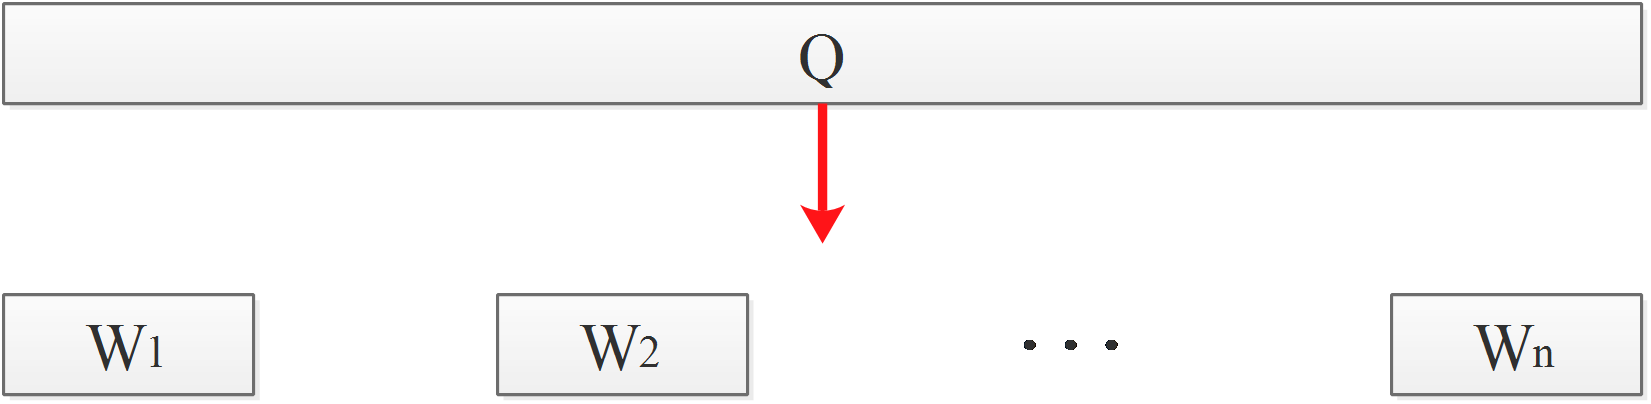
\includegraphics[width=\columnwidth]{rk7.png}
		\end{column}
	\end{columns}
\end{frame}

\begin{frame}{ETS}
	\begin{columns}[t]
		\begin{column}{0.8\textwidth} % 横幅の30%
			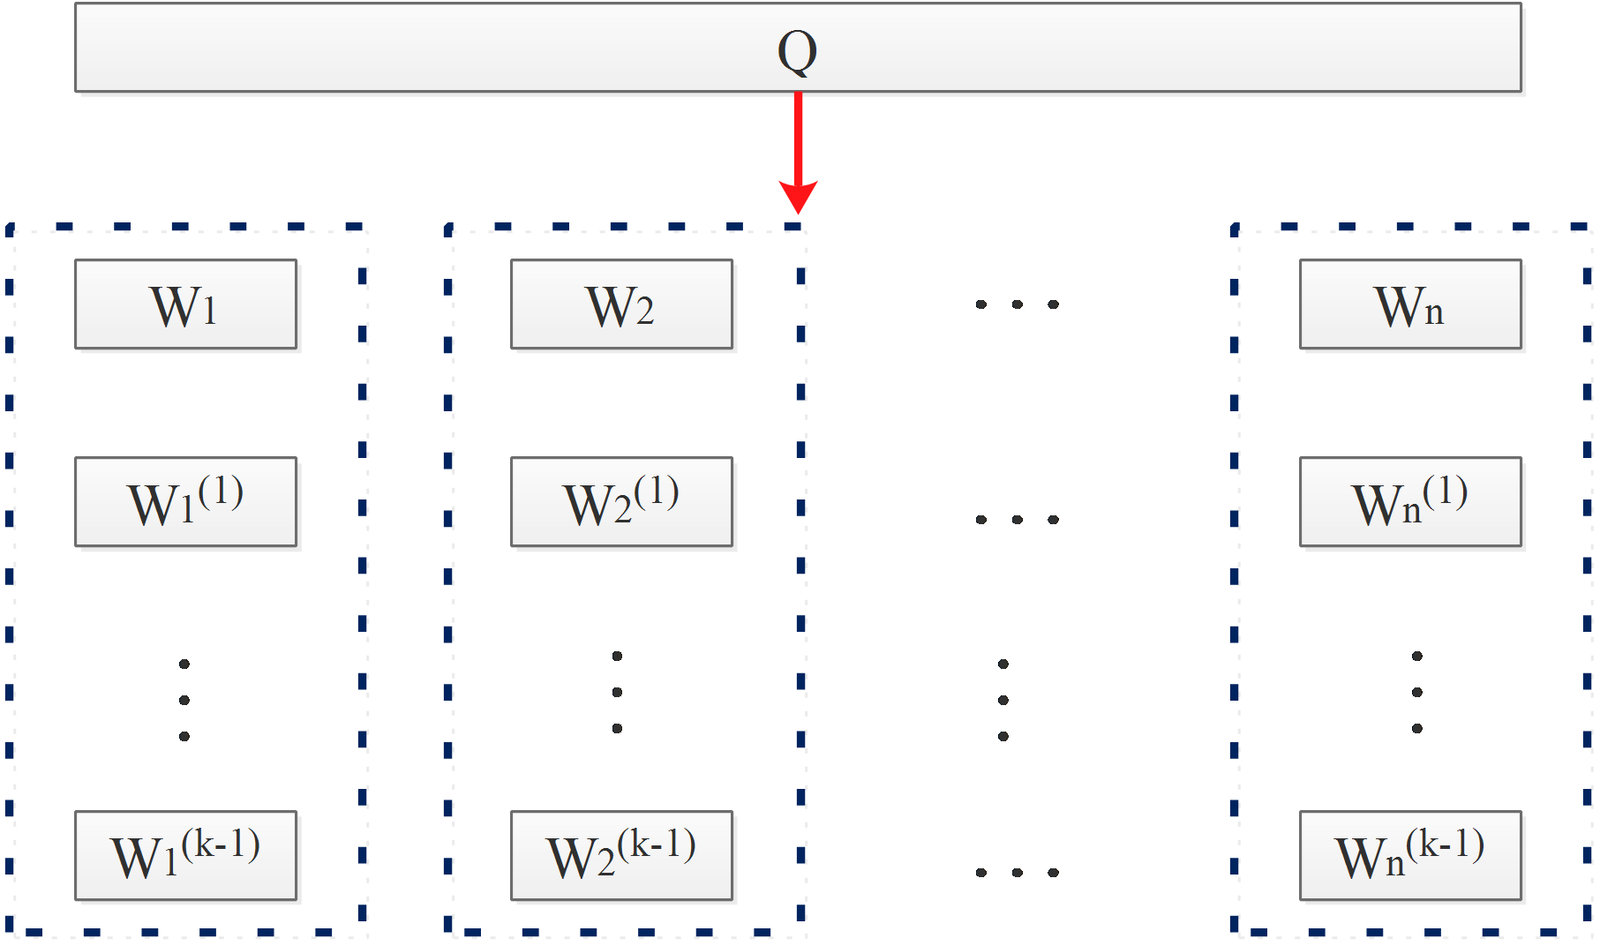
\includegraphics[width=\columnwidth]{rk8.png}
		\end{column}
	\end{columns}
	\begin{block}{}
		真の質問である可能性がある質問数:$K \textcolor{red}\rightarrow K^n$	
	\end{block}
\end{frame}

\begin{frame}{質問検索}
\fontsize{12pt}{7.2}\selectfont
	\begin{columns}[t]
		\begin{column}{0.8\textwidth} % 横幅の30%
			
\includegraphics[width=\columnwidth]{rk9.png}
		\end{column}
	\end{columns}
	\begin{block}{}
		単語$W_i$に対して文章$d_j$のスコア:$s_{ij}$ \\
		質問$Q$に対して文章$d_j$のスコア:$s_{j}=\sum_{i \in Q}s_{ij}$ \\
		スコアが上位$m$個にある文章を質問$Q$の検索結果として返す
	\end{block}
\end{frame}

\begin{frame}{質問検索-ETS}
\fontsize{12pt}{7.2}\selectfont
	\begin{minipage}[c]{0.65\textwidth}
			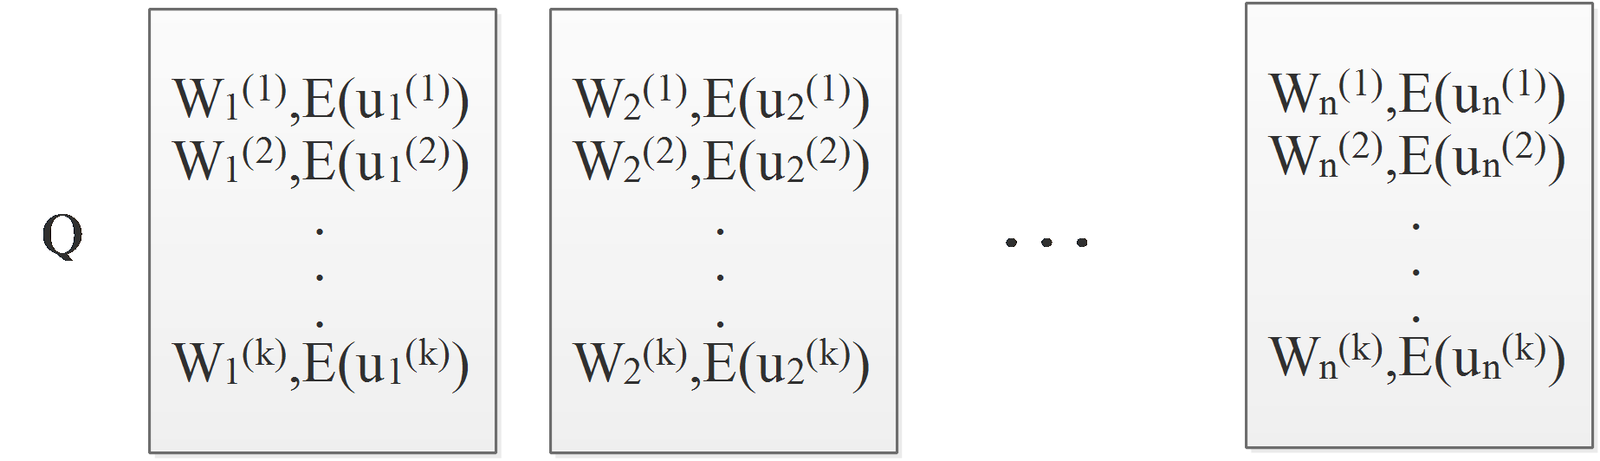
\includegraphics[width=\columnwidth]{rk10.png}
	\end{minipage}%
	\begin{minipage}[c]{0.25\textwidth}
			$$\,\,u_i^{(k)}=\left\{
			\begin{aligned}
			0& \, i,k \notin Q^* \\
			1& \, i,k \in Q^*
			\end{aligned}
			\right.
			$$
	\end{minipage}
	\begin{block}{}
		単語$W_i^{(k)}$に対して文章$d_j$のスコア:$s'_{ikj}=E(u_i^{(k)})^{(s_{ikj})}$ \\
		質問$Q$に対して文章$d_j$のスコア:$s_{j}=\prod_{i,k \in Q}s'_{ikj}$ \\
		スコアが$0$ではない文章を全部返す
	\end{block}
\end{frame}

\begin{frame}{Wordnet}
\fontsize{12pt}{7.2}\selectfont
	\begin{columns}[t]
		\begin{column}{1.0\textwidth} % 横幅の30%
			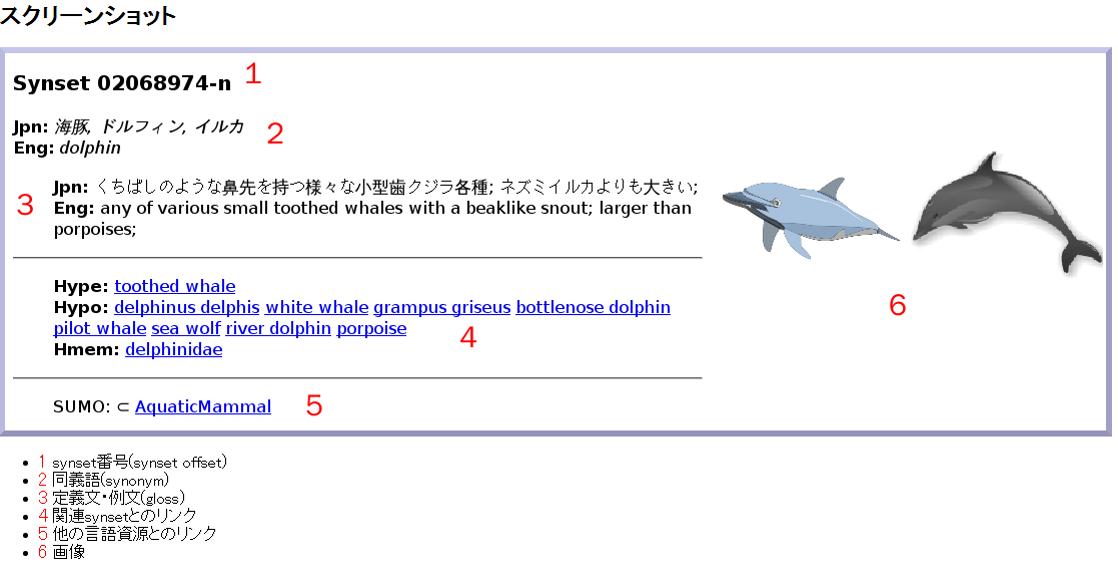
\includegraphics[width=\columnwidth]{photo14.png}
		\end{column}
	\end{columns}
	\begin{block}{}
		単語を意味ごとに分類するデータベース \\
		リンクを持つsynsetを隣に並ぶことにより、すべての名詞を一列に並ぶ$:t_1 \, t_2 \, t_3 \, \dots \, t_{1000}$
	\end{block}
\end{frame}

\begin{frame}{単語列}
	\begin{columns}[t]
		\begin{column}{1.0\textwidth} % 横幅の30%
			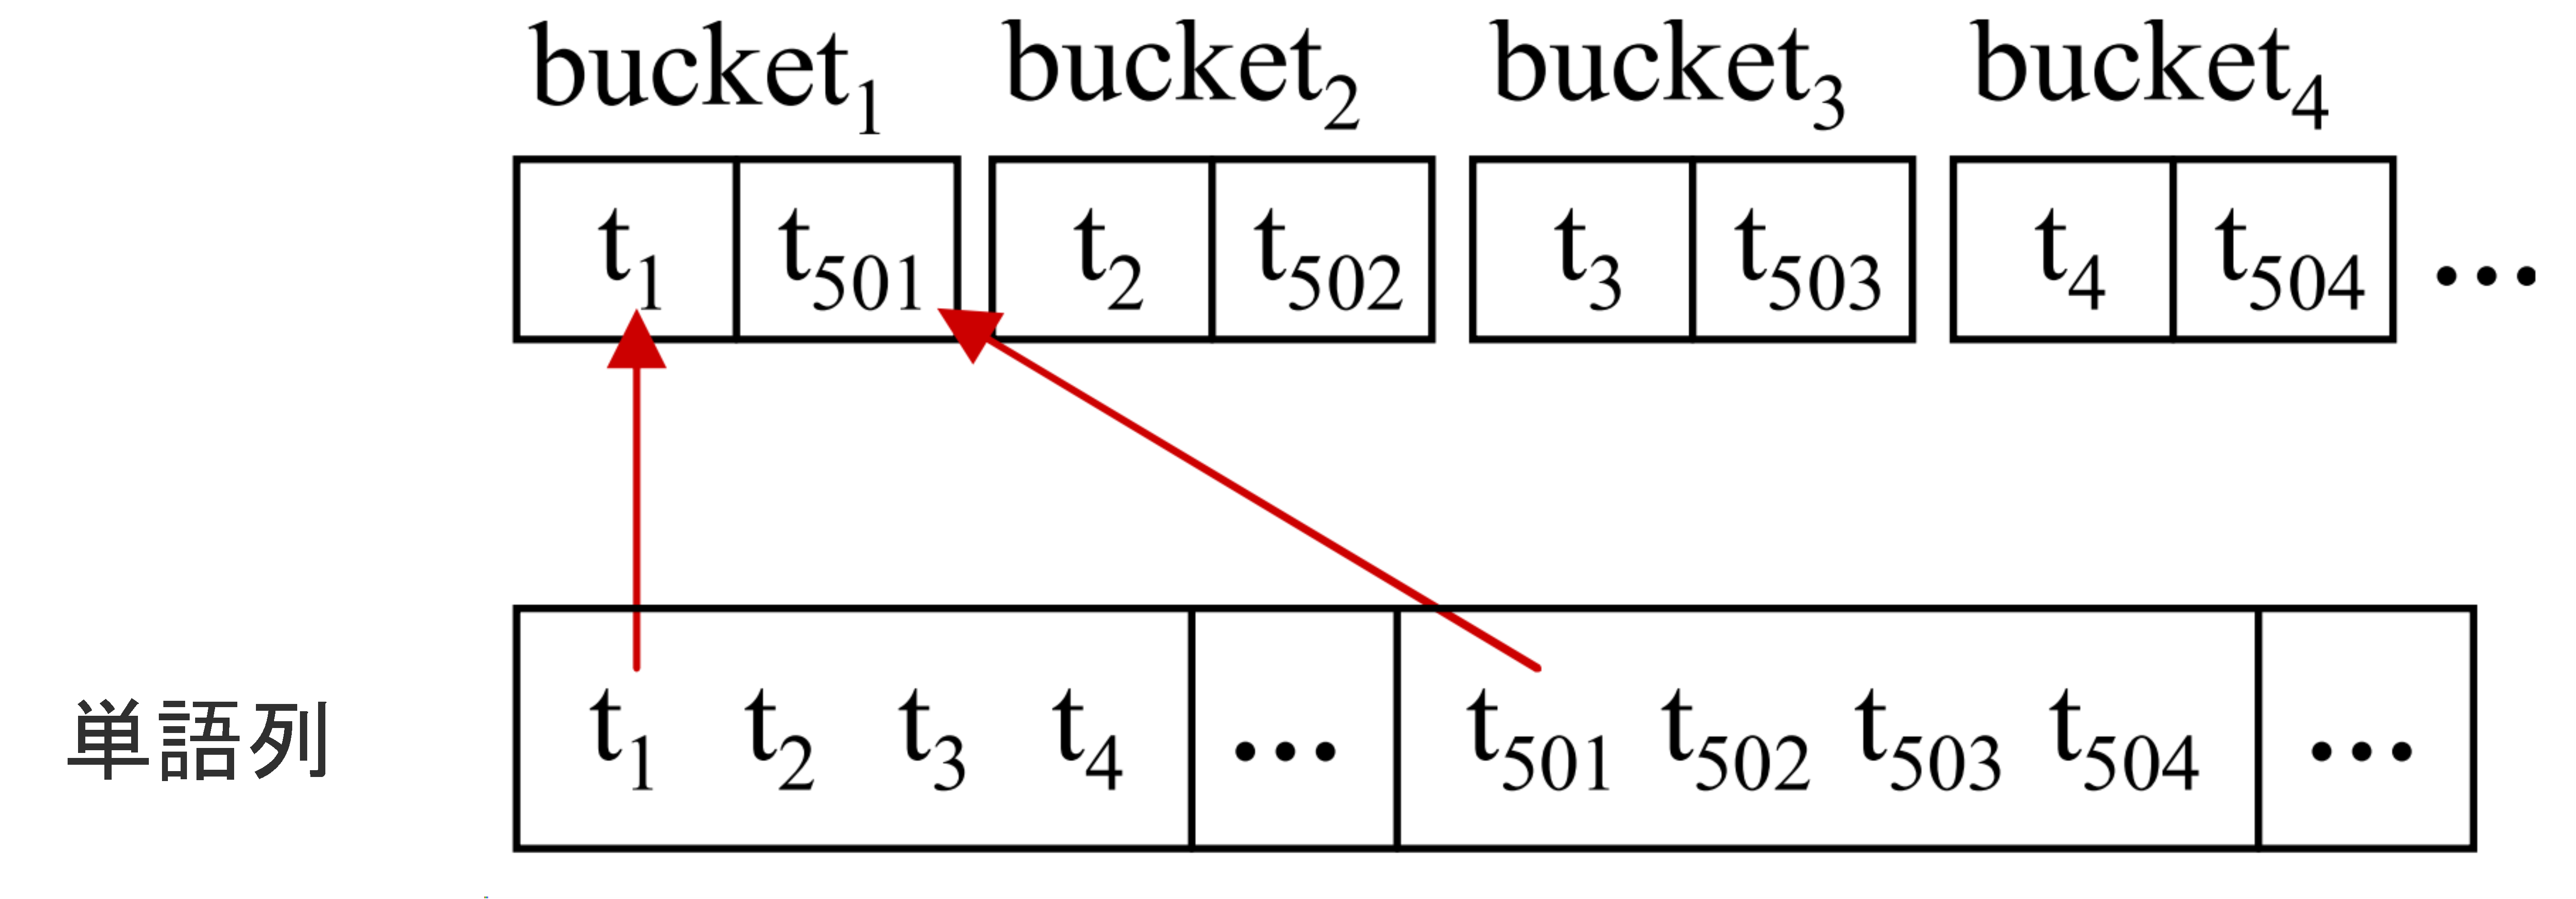
\includegraphics[width=\columnwidth]{rk11.png}
		\end{column}
	\end{columns}
\end{frame}

\begin{frame}{Wordnet}
\fontsize{12pt}{7.2}\selectfont
	\begin{columns}[t]
		\begin{column}{1.0\textwidth} % 横幅の30%
			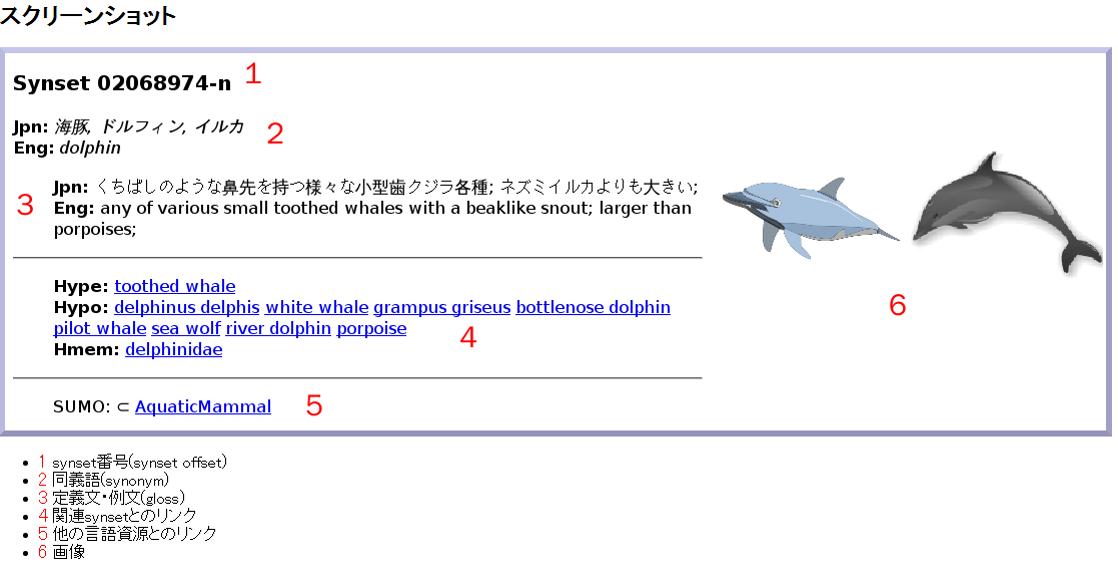
\includegraphics[width=\columnwidth]{photo14.png}
		\end{column}
	\end{columns}
	\begin{block}{}
		実体/entity以外全部の名詞の上位語が唯一に存在する \\
		上下位関係を枝とすると、Wordnet中の名詞が木の形になる
	\end{block}
\end{frame}

\begin{frame}{Wordnet}
	\begin{columns}[t]
		\begin{column}{1.0\textwidth} % 横幅の30%
			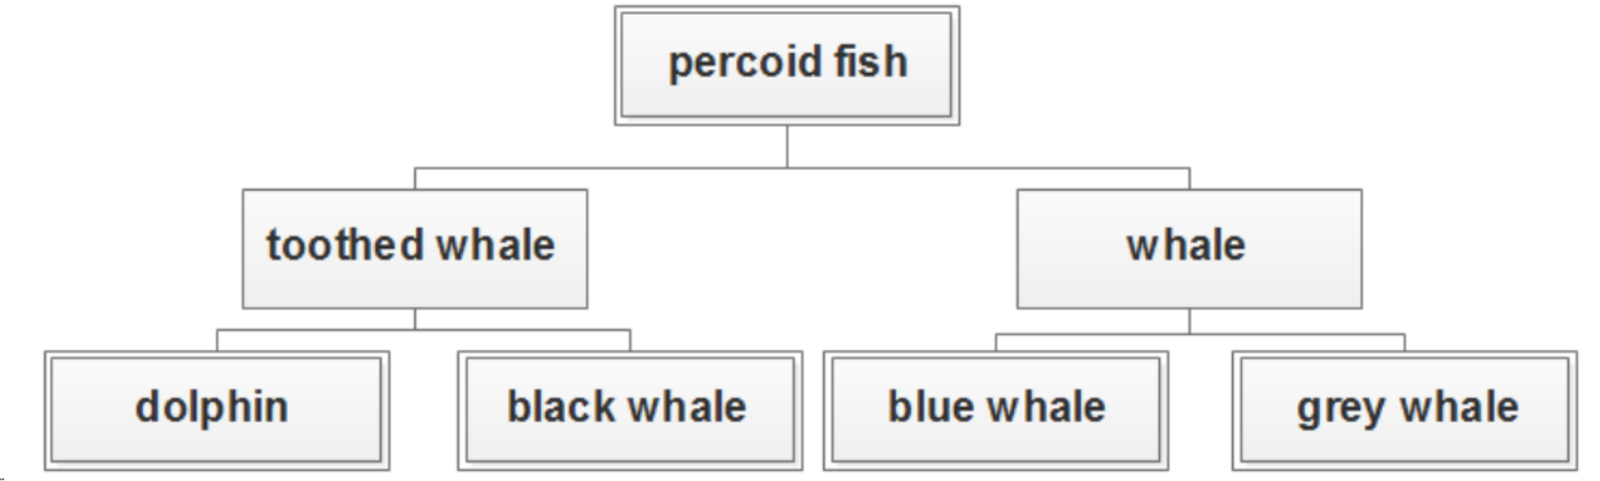
\includegraphics[width=\columnwidth]{rk12.png}
		\end{column}
	\end{columns}
\end{frame}

\begin{frame}{Wordnet}
	\begin{columns}[t]
		\begin{column}{0.8\textwidth} % 横幅の30%
			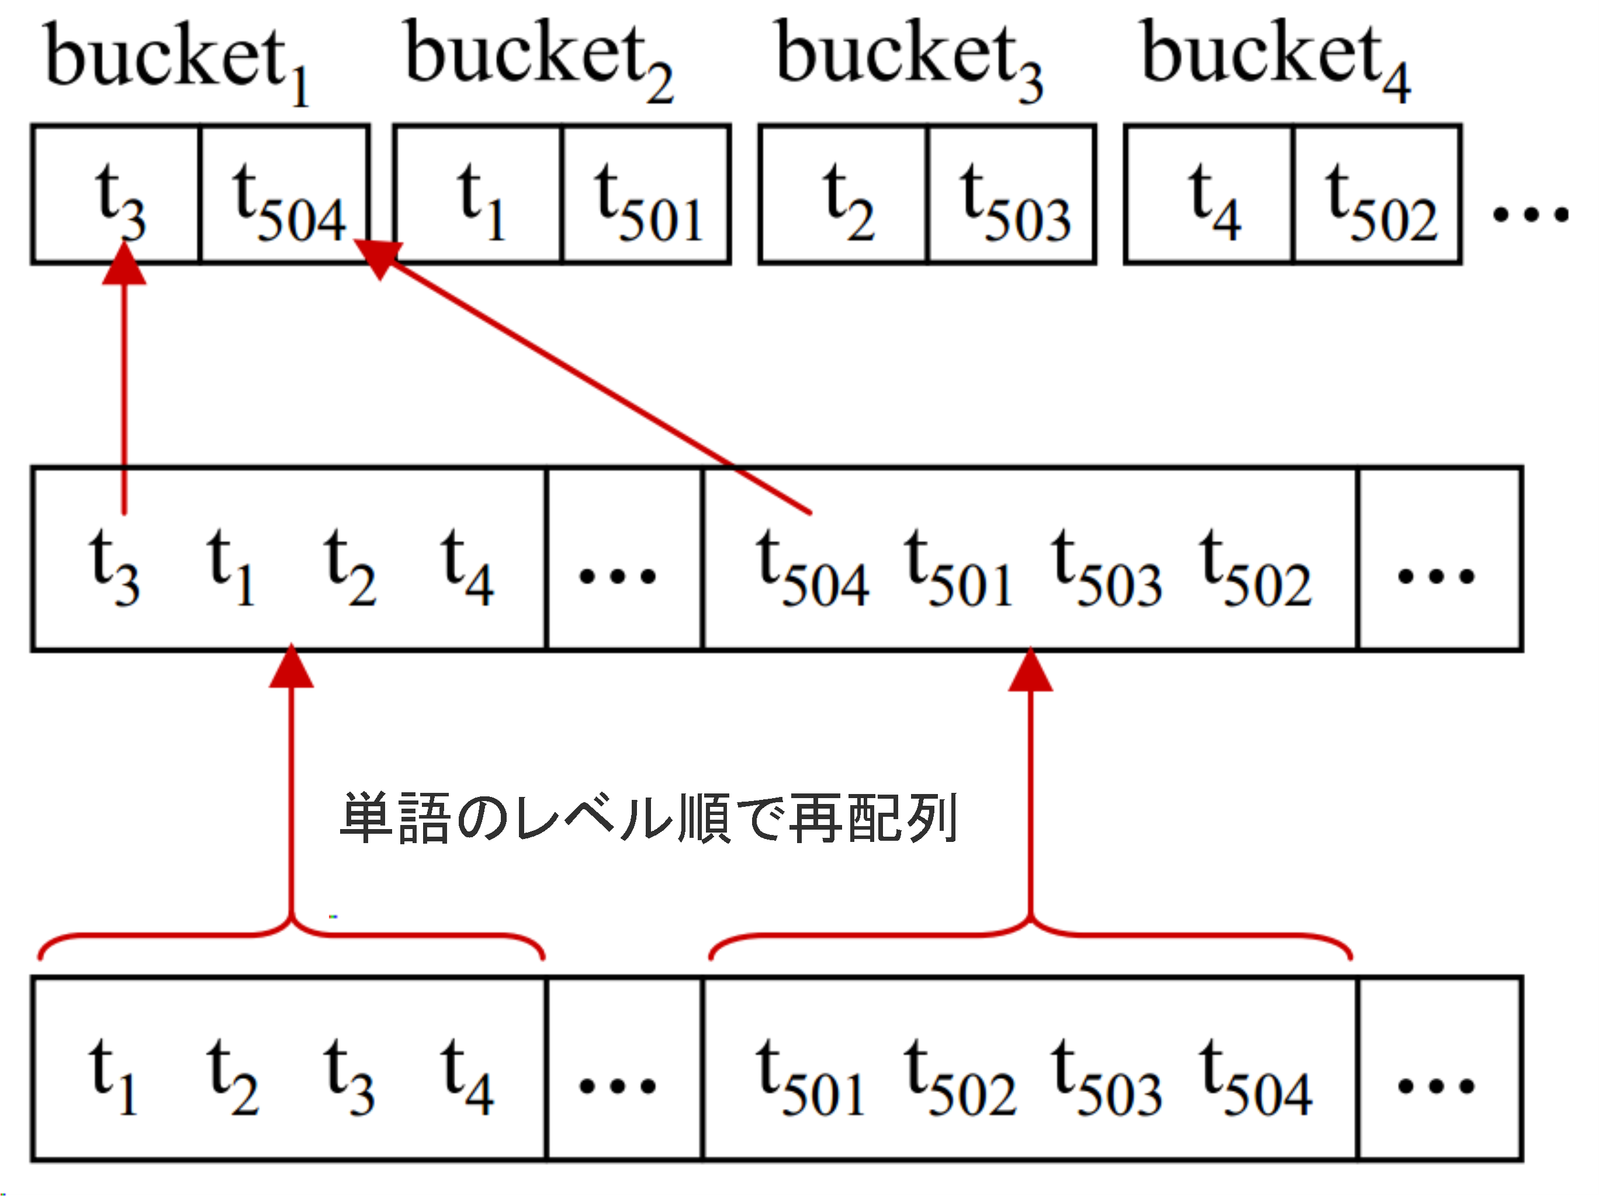
\includegraphics[width=\columnwidth]{rk13.png}
		\end{column}
	\end{columns}
\end{frame}

\section{プライバシー分析}
\begin{frame}{クエリ分析}
	\begin{exampleblock}{}
	\fontsize{5pt}{7.2}\selectfont
		\begin{tabular}{cccccccccccccccc}
		\noalign{\hrule height 1pt}
		メタノール & 水蒸気 & 反応 & 水素 & 透過 & 膜 & $\dots$ & 燃料 \\
		\hline
		衡平 & グンバイムシ & 水力 & 上唇 & ドアロック & 沈殿 & $\dots$  & ベーキングパウダー \\
		ルシタニア & ファースト & テアトル & 水素 & 認知心理学 & 膜 & $\dots$  & 運転者 \\
		メタノール & 水蒸気 & 反応 & 長引かせること & 透過 & 組織図 & $\dots$  & 燃料 \\
		分限者 & カランツ & 意味合 & 発明品 & イーサネットケーブル & 原稿 & $\dots$  & 黒泥土 \\
		\noalign{\hrule height 1pt}
		\end{tabular}
	\end{exampleblock}
	\begin{block}{}
		真の質問の単語は全部燃料電池と関係あるが、ダミー単語の意味がバラバラである \\ もし単語が意味によって分類できるなら、燃料電池と関係がある単語が他のクラスに属する単語の数より多いことが考えられる
	\end{block}
\end{frame}

\begin{frame}{Latent Semantic Analysis}
    \begin{columns}[c]
        \begin{column}{1.0\textwidth} % 横幅の30%
            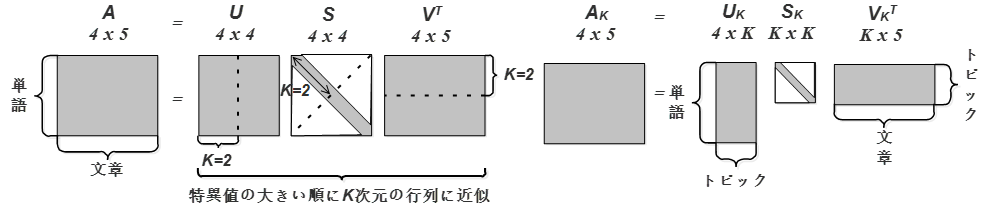
\includegraphics[width=\columnwidth]{photo11.png}
		\end{column}
    \end{columns}
	\begin{block}{潜在的意味インデキシング}
	\fontsize{12pt}{7.2}\selectfont
		単語$\cdot$文書行列$A$を特異値分解$A = USV^T$し、$U$、$S$、$V$	の各列ベクトルを特異値が大きい順に
		$K$個用いて$A$の低ランク近似$A_K=U_KS_KV_{K}^T$を得る。 \\
		このように低ランク分解によって、単語とトピックの関係を分析することができる \\
		今回は同じ分類に属する全部の文章を1文章としてLSAを行った
	\end{block}
\end{frame}


\begin{frame}{主意味攻撃}
	\begin{exampleblock}{}
	\fontsize{5pt}{7.2}\selectfont
		\begin{tabular}{cccccccccccccccc}
		\noalign{\hrule height 1pt}
		メタノール & 水蒸気 & 反応 & 水素 & 透過 & 膜 & $\dots$ & 燃料 \\
		\hline
		衡平 & グンバイムシ & 水力 & 上唇 & ドアロック & 沈殿 & $\dots$  & ベーキングパウダー \\
		ルシタニア & ファースト & テアトル & 水素 & 認知心理学 & 膜 & $\dots$  & 運転者 \\
		メタノール & 水蒸気 & 反応 & 長引かせること & 透過 & 組織図 & $\dots$  & 燃料 \\
		分限者 & カランツ & 意味合 & 発明品 & イーサネットケーブル & 原稿 & $\dots$  & 黒泥土 \\
		\noalign{\hrule height 1pt}
		\end{tabular}
	\end{exampleblock}
	\begin{block}{主意味攻撃}
	\fontsize{12pt}{7.2}\selectfont
	\begin{algorithmic}[1]
		\REQUIRE 質問:$Q=\{t_i\},$単語のトピックベクトル集合$L=\{\ell_i\}$
		\STATE $R=\phi, \, \ell=0$
		\STATE $\ell=\sum_{t_i \in Q}\ell_{t_i}$
		\STATE $maintopic=argmax_j \ell[j]$
		\FORALL {$bk_k \in Q $}
		\STATE $R=R \cup max_{t_i}q_{t_i}[maintopic]$
		\ENDFOR
		\RETURN $R$
	\end{algorithmic}
	\end{block}
\end{frame}

\begin{frame}{プライバシー分析}
	\begin{center}
		\begin{tabular}{|c|c|}
		\noalign{\hrule height 1pt}
		重複を除いた単語数 & $2,973,096$  \\
		文章数 & $3,496,253$ \\
		質問数 & $2,908$ \\
		質問平均単語数 & $21.0$ \\
		主意味攻撃成功率 & $90.1\%$ \\
		\noalign{\hrule height 1pt}
		\end{tabular}
	\end{center}
\end{frame}

\section{参考文献}
\begin{frame}[t,allowframebreaks]{Bibliography}
\fontsize{8pt}{7.2}\selectfont
\bibliographystyle{alpha}
\bibliography{zotero}
\end{frame}

\end{document}
